\begin{figure}[t]
\centering
\begin{minipage}[t]{0.23\textwidth}
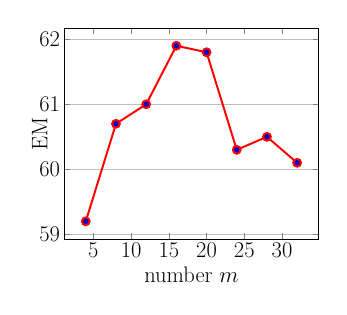
\begin{tikzpicture}[scale=0.47]
    \begin{axis}[
        xlabel=number $m$,
        ylabel=EM,
        y label style={at={(-0.05,0.5)}},
        ymajorgrids=true,
        font=\LARGE,
        ]
        \addplot+[color=red,line width=1.5pt,mark size=3pt] coordinates {
            (4,59.2)
            (8,60.7)
            (12,61.0)
            (16,61.9)
            (20,61.8)
            (24,60.3)
            (28,60.5)
            (32,60.1)
        };
    \end{axis}
\end{tikzpicture}
\caption{Impact of passage-level embedding number}
\label{fig:global token number}
\end{minipage}
\begin{minipage}[t]{0.23\textwidth}
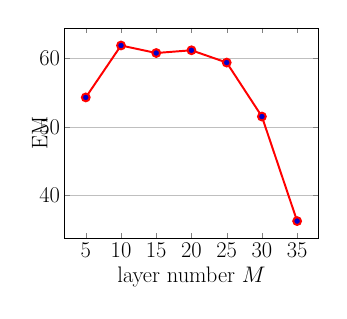
\begin{tikzpicture}[scale=0.47]
    \begin{axis}[
        xlabel=layer number $M$,
        ylabel=EM,
        y label style={at={(-0.05,0.5)}},
        ymajorgrids=true,
        font=\LARGE,
        % ymin=0.12,
        % ymax=0.15,
        ]
        \addplot+ [color=red,line width=1.5pt,mark size=3pt] coordinates {
            (5,54.3)
            (10,61.9)
            (15,60.8)
            (20,61.2)
            (25,59.4)
            (30,51.5)
            (35,36.2)
        };
    \end{axis}
\end{tikzpicture}
\caption{Impact of cyclic passage-question co-encoding layers number}
\label{fig:local encoding layers number}
\end{minipage}
\end{figure}